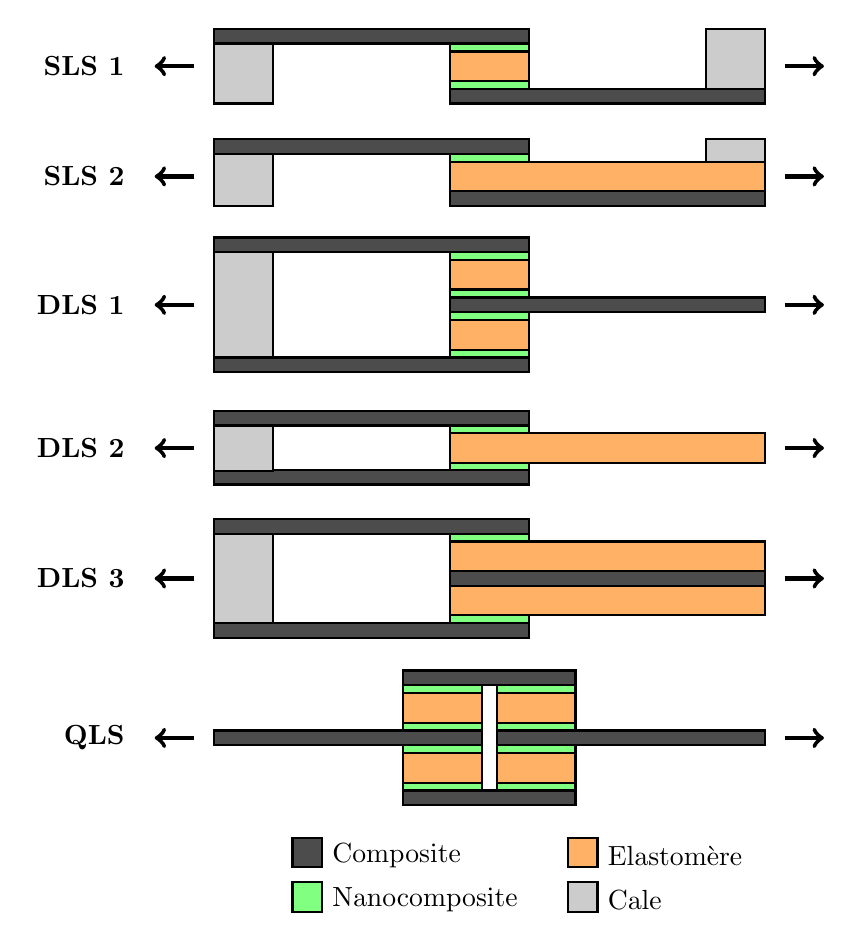
\begin{tikzpicture}[scale=0.5, thick]

%Dimensons générales
\def \overlap{2}
\def \espacevert{1}

%Dimensions composite
\def \lcomp{8}
\def \tcomp{0.375}

%Épaisseur de l'élément résistif
\def \tele{0.2}

%Épaisseur de l'élastomère
\def \tela{0.75}

%Dimensions de la calle
\def \lcalle{1.5}

%Position et taille des annotations
\def \lforce{1}
\def \gapforce{0.5}
\def \gaptexte{0.375}
\def \legende{0.75}
\def \gapscie{0.375}
\def \midgap{0.375}

%Couleurs
\def \colcomp{black!70}
\def \colele{green!50}
\def \colelas{orange!60}
\def \colcalle{black!20}


%\begin{scope}[shift={(0,21)}]
%	%Plaques
%	\draw[black,fill=\colcomp] (0,0) -- ++(0,\tcomp) -- ++(\lcomp,0) -- ++(0,-\tcomp) -- cycle; %Single shear haut
%	\draw[black,fill=\colcomp] (\lcomp-\overlap,-\tele-\tcomp) -- ++(0,\tcomp) -- ++(\lcomp,0) -- ++(0,-\tcomp) -- cycle; %Single shear bas
%	
%	%Éléments chauffants
%	\draw[black,fill=\colele] (\lcomp-\overlap,-\tele) -- ++(0,\tele) -- ++(\overlap,0) -- ++(0,-\tele) -- cycle; %Single shear
%	
%	%Calles
%	\draw[black,fill=\colcalle] (0,0) -- ++(0,-\tele-\tcomp) -- ++(\lcalle,0) -- ++(0,\tele+\tcomp) -- cycle; % calle 1
%	\draw[black,fill=\colcalle] (2*\lcomp-\overlap-\lcalle,\tcomp) -- ++(0,-\tele-\tcomp) -- ++(\lcalle,0) -- ++(0,\tele+\tcomp) -- cycle; % calle 2
%	
%	%Lignes de force
%	\begin{scope}[ultra thick]
%	\draw [->] (-\gapforce,-.5*\tele) -- ++(-\lforce,0);
%	\draw [->] (2*\lcomp-\overlap+\gapforce,-.5*\tele) -- ++(\lforce,0);
%	\end{scope}
%	
%	%Identification de l'éprouvette
%	\draw (-\lforce-2*\gapforce,-.5*\tele) node[left]{\textbf{SLS}};
%\end{scope}

\begin{scope}[shift={(0,18.8)}]
	%Plaques
	\draw[black,fill=\colcomp] (0,0) -- ++(0,\tcomp) -- ++(\lcomp,0) -- ++(0,-\tcomp) -- cycle; %single shear haut 1
	\draw[black,fill=\colcomp] (\lcomp-\overlap,-2*\tele-\tcomp-\tela) -- ++(0,\tcomp) -- ++(\lcomp,0) -- ++(0,-\tcomp) -- cycle; %single shear bas 2
	
	%Éléments chauffants
	\draw[black,fill=\colele] (\lcomp-\overlap,-\tele) -- ++(0,\tele) -- ++(\overlap,0) -- ++(0,-\tele) -- cycle; %single shear haut 2
	\draw[black,fill=\colele] (\lcomp-\overlap,-2*\tele-\tela) -- ++(0,\tele) -- ++(\overlap,0) -- ++(0,-\tele) -- cycle; %single shear bas 2
	
	%Élastomère
	\draw[black,fill=\colelas] (\lcomp-\overlap,-\tela-\tele) -- ++(0,\tela) -- ++(\overlap,0) -- ++(0,-\tela) -- cycle; % elastomère 2

	%Calles
	\draw[black,fill=\colcalle] (0,0) -- ++(0,-2*\tele-\tcomp-\tela) -- ++(\lcalle,0) -- ++(0,2*\tele+\tcomp+\tela) -- cycle; % calle 1
	\draw[black,fill=\colcalle] (2*\lcomp-\overlap-\lcalle,\tcomp) -- ++(0,-2*\tele-\tcomp-\tela) -- ++(\lcalle,0) -- ++(0,2*\tele+\tcomp+\tela) -- cycle; % calle 2
	
	%Lignes de force
	\begin{scope}[ultra thick]
	\draw [->] (-\gapforce,-\tele-0.5*\tela) -- ++(-\lforce,0);
	\draw [->] (2*\lcomp-\overlap+\gapforce,-\tele-0.5*\tela) -- ++(\lforce,0);
	\end{scope}
	
	%Identification de l'éprouvette
	\draw (-\lforce-2*\gapforce,-\tele-0.5*\tela) node[left]{\textbf{SLS 1}};
\end{scope}

\begin{scope}[shift={(0,16)}] 
	%Plaques
	\draw[black,fill=\colcomp] (0,0) -- ++(0,\tcomp) -- ++(\lcomp,0) -- ++(0,-\tcomp) -- cycle; %single shear haut 1
	\draw[black,fill=\colcomp] (\lcomp-\overlap,-\tele-\tcomp-\tela) -- ++(0,\tcomp) -- ++(\lcomp,0) -- ++(0,-\tcomp) -- cycle; %single shear bas 2
	
	%Éléments chauffants
	\draw[black,fill=\colele] (\lcomp-\overlap,-\tele) -- ++(0,\tele) -- ++(\overlap,0) -- ++(0,-\tele) -- cycle; %single shear haut 2

	%Élastomère
	\draw[black,fill=\colelas] (\lcomp-\overlap,-\tela-\tele) -- ++(0,\tela) -- ++(\lcomp,0) -- ++(0,-\tela) -- cycle; % elastomère 2

	%Calles
	\draw[black,fill=\colcalle] (0,0) -- ++(0,-\tele-\tcomp-\tela) -- ++(\lcalle,0) -- ++(0,\tele+\tcomp+\tela) -- cycle; % calle 1
	\draw[black,fill=\colcalle] (2*\lcomp-\overlap-\lcalle,\tcomp) -- ++(0,-\tele-\tcomp) -- ++(\lcalle,0) -- ++(0,\tele+\tcomp) -- cycle; % calle 2
	
	%Lignes de force
	\begin{scope}[ultra thick]
	\draw [->] (-\gapforce,-\tele-0.5*\tela) -- ++(-\lforce,0);
	\draw [->] (2*\lcomp-\overlap+\gapforce,-\tele-0.5*\tela) -- ++(\lforce,0);
	\end{scope}
	
	%Identification de l'éprouvette
	\draw (-\lforce-2*\gapforce,-\tele-0.5*\tela) node[left]{\textbf{SLS 2}};
\end{scope}


\begin{scope}[shift={(0,13.5)}]
	%Plaques
	\draw[black,fill=\colcomp] (0,0) -- ++(0,\tcomp) -- ++(\lcomp,0) -- ++(0,-\tcomp) -- cycle; %dual shear haut
	\draw[black,fill=\colcomp] (\lcomp-\overlap,-2*\tele-\tcomp-\tela) -- ++(0,\tcomp) -- ++(\lcomp,0) -- ++(0,-\tcomp) -- cycle; %dual shear milieu
	\draw[black,fill=\colcomp] (0,-2*\tcomp-4*\tele-2*\tela) -- ++(0,\tcomp) -- ++(\lcomp,0) -- ++(0,-\tcomp) -- cycle; %dual shear bas
	
	%Éléments chauffants
	\draw[black,fill=\colele] (\lcomp-\overlap,-\tele) -- ++(0,\tele) -- ++(\overlap,0) -- ++(0,-\tele) -- cycle; %dual shear haut 1
	\draw[black,fill=\colele] (\lcomp-\overlap,-2*\tele-\tela) -- ++(0,\tele) -- ++(\overlap,0) -- ++(0,-\tele) -- cycle; %dual shear haut 2
	\draw[black,fill=\colele] (\lcomp-\overlap,-3*\tele-\tela-\tcomp) -- ++(0,\tele) -- ++(\overlap,0) -- ++(0,-\tele) -- cycle; %dual shear bas 1
	\draw[black,fill=\colele] (\lcomp-\overlap,-4*\tele-2*\tela-\tcomp) -- ++(0,\tele) -- ++(\overlap,0) -- ++(0,-\tele) -- cycle; %dual shear bas 2
	
	%Élastomère
	\draw[black,fill=\colelas] (\lcomp-\overlap,-\tela-\tele) -- ++(0,\tela) -- ++(\overlap,0) -- ++(0,-\tela) -- cycle; % elastomère haut
	\draw[black,fill=\colelas] (\lcomp-\overlap,-2*\tela-3*\tele-\tcomp) -- ++(0,\tela) -- ++(\overlap,0) -- ++(0,-\tela) -- cycle; % elastomère bas
	
	%Calle
	\draw[black,fill=\colcalle] (0,0) -- ++(0,-4*\tele-2*\tela-\tcomp) -- ++(\lcalle,0) -- ++(0,4*\tele+2*\tela+\tcomp) -- cycle; % calle
	
	%Lignes de force
	\begin{scope}[ultra thick]
	\draw [->] (-\gapforce,-2*\tele-\tela-0.5*\tcomp) -- ++(-\lforce,0);
	\draw [->] (2*\lcomp-\overlap+\gapforce,-2*\tele-\tela-0.5*\tcomp) -- ++(\lforce,0);
	\end{scope}
	
	%Identification de l'éprouvette
	\draw (-\lforce-2*\gapforce,-2*\tele-\tela-0.5*\tcomp) node[left]{\textbf{DLS 1}};
\end{scope}


\begin{scope}[shift={(0,9.1)}] 
	%Plaques
	\draw[black,fill=\colcomp] (0,0) -- ++(0,\tcomp) -- ++(\lcomp,0) -- ++(0,-\tcomp) -- cycle; %dual shear haut
	\draw[black,fill=\colcomp] (0,-2*\tcomp-\tela) -- ++(0,\tcomp) -- ++(\lcomp,0) -- ++(0,-\tcomp) -- cycle; %dual shear bas
	
	%Éléments chauffants
	\draw[black,fill=\colele] (\lcomp-\overlap,-\tele) -- ++(0,\tele) -- ++(\overlap,0) -- ++(0,-\tele) -- cycle; %dual shear haut 1
	\draw[black,fill=\colele] (\lcomp-\overlap,-\tela-\tcomp) -- ++(0,\tele) -- ++(\overlap,0) -- ++(0,-\tele) -- cycle; %dual shear bas 2
	
	%Élastomère
	\draw[black,fill=\colelas] (\lcomp-\overlap,-\tela-\tele) -- ++(0,\tela) -- ++(\lcomp,0) -- ++(0,-\tela) -- cycle; % elastomère haut
	
	%Calle
	\draw[black,fill=\colcalle] (0,0) -- ++(0,-2*\tele-\tela) -- ++(\lcalle,0) -- ++(0,2*\tele+\tela) -- cycle; % calle
	
	%Lignes de force
	\begin{scope}[ultra thick]
	\draw [->] (-\gapforce,-\tele-0.5*\tela) -- ++(-\lforce,0);
	\draw [->] (2*\lcomp-\overlap+\gapforce,-\tele-0.5*\tela) -- ++(\lforce,0);
	\end{scope}
	
	%Identification de l'éprouvette
	\draw (-\lforce-2*\gapforce,-\tele-0.5*\tela) node[left]{\textbf{DLS 2}};
\end{scope}


\begin{scope}[shift={(0,6.35)}] 
	%Plaques
	\draw[black,fill=\colcomp] (0,0) -- ++(0,\tcomp) -- ++(\lcomp,0) -- ++(0,-\tcomp) -- cycle; %dual shear haut
	\draw[black,fill=\colcomp] (\lcomp-\overlap,-\tele-\tcomp-\tela) -- ++(0,\tcomp) -- ++(\lcomp,0) -- ++(0,-\tcomp) -- cycle; %dual shear milieu
	\draw[black,fill=\colcomp] (0,-2*\tcomp-2*\tele-2*\tela) -- ++(0,\tcomp) -- ++(\lcomp,0) -- ++(0,-\tcomp) -- cycle; %dual shear bas
	
	%Éléments chauffants
	\draw[black,fill=\colele] (\lcomp-\overlap,-\tele) -- ++(0,\tele) -- ++(\overlap,0) -- ++(0,-\tele) -- cycle; %dual shear haut 1
	\draw[black,fill=\colele] (\lcomp-\overlap,-2*\tele-2*\tela-\tcomp) -- ++(0,\tele) -- ++(\overlap,0) -- ++(0,-\tele) -- cycle; %dual shear bas 2
	
	%Élastomère
	\draw[black,fill=\colelas] (\lcomp-\overlap,-\tela-\tele) -- ++(0,\tela) -- ++(\lcomp,0) -- ++(0,-\tela) -- cycle; % elastomère haut
	\draw[black,fill=\colelas] (\lcomp-\overlap,-2*\tela-1*\tele-\tcomp) -- ++(0,\tela) -- ++(\lcomp,0) -- ++(0,-\tela) -- cycle; % elastomère bas
	
	%Calle
	\draw[black,fill=\colcalle] (0,0) -- ++(0,-2*\tele-2*\tela-\tcomp) -- ++(\lcalle,0) -- ++(0,2*\tele+2*\tela+\tcomp) -- cycle; % calle
	
	%Lignes de force
	\begin{scope}[ultra thick]
	\draw [->] (-\gapforce,-\tele-\tela-0.5*\tcomp) -- ++(-\lforce,0);
	\draw [->] (2*\lcomp-\overlap+\gapforce,-\tele-\tela-0.5*\tcomp) -- ++(\lforce,0);
	\end{scope}
	
	%Identification de l'éprouvette
	\draw (-\lforce-2*\gapforce,-\tele-\tela-0.5*\tcomp) node[left]{\textbf{DLS 3}};
\end{scope}


\begin{scope}[shift={(0,2.5)}]
	%Plaques
	\draw[black,fill=\colcomp] (\lcomp-1.5*\overlap-0.5*\midgap,0) -- ++(0,\tcomp) -- ++(2*\overlap+\midgap,0) -- ++(0,-\tcomp) -- cycle; %quad shear haut
	\draw[black,fill=\colcomp] (0,-2*\tele-\tcomp-\tela) -- ++(0,\tcomp) -- ++(\lcomp-0.5*\overlap-0.5*\midgap,0) -- ++(0,-\tcomp) -- cycle; %quad shear milieu 1
	\draw[black,fill=\colcomp] (\lcomp-0.5*\overlap+0.5*\midgap,-2*\tele-\tcomp-\tela) -- ++(0,\tcomp) -- ++(\lcomp-0.5*\overlap-0.5*\midgap,0) -- ++(0,-\tcomp) -- cycle; %quad shear milieu 2
	\draw[black,fill=\colcomp] (\lcomp-1.5*\overlap-0.5*\midgap,-2*\tcomp-4*\tele-2*\tela) -- ++(0,\tcomp) -- ++(2*\overlap+\midgap,0) -- ++(0,-\tcomp) -- cycle; %quad shear bas
	
	%Éléments chauffants 
	
	%gauche
	\draw[black,fill=\colele] (\lcomp-1.5*\overlap-0.5*\midgap,-\tele) -- ++(0,\tele) -- ++(\overlap,0) -- ++(0,-\tele) -- cycle; %quad shear haut 1
	\draw[black,fill=\colele] (\lcomp-1.5*\overlap-0.5*\midgap,-2*\tele-\tela) -- ++(0,\tele) -- ++(\overlap,0) -- ++(0,-\tele) -- cycle; %quad shear haut 2
	\draw[black,fill=\colele] (\lcomp-1.5*\overlap-0.5*\midgap,-3*\tele-\tela-\tcomp) -- ++(0,\tele) -- ++(\overlap,0) -- ++(0,-\tele) -- cycle; %quad shear bas 1
	\draw[black,fill=\colele] (\lcomp-1.5*\overlap-0.5*\midgap,-4*\tele-2*\tela-\tcomp) -- ++(0,\tele) -- ++(\overlap,0) -- ++(0,-\tele) -- cycle; %quad shear bas 2
	
	%droite
	\draw[black,fill=\colele] (\lcomp-0.5*\overlap+0.5*\midgap,-\tele) -- ++(0,\tele) -- ++(\overlap,0) -- ++(0,-\tele) -- cycle; %quad shear haut 1
	\draw[black,fill=\colele] (\lcomp-0.5*\overlap+0.5*\midgap,-2*\tele-\tela) -- ++(0,\tele) -- ++(\overlap,0) -- ++(0,-\tele) -- cycle; %quad shear haut 2
	\draw[black,fill=\colele] (\lcomp-0.5*\overlap+0.5*\midgap,-3*\tele-\tela-\tcomp) -- ++(0,\tele) -- ++(\overlap,0) -- ++(0,-\tele) -- cycle; %quad shear bas 1
	\draw[black,fill=\colele] (\lcomp-0.5*\overlap+0.5*\midgap,-4*\tele-2*\tela-\tcomp) -- ++(0,\tele) -- ++(\overlap,0) -- ++(0,-\tele) -- cycle; %quad shear bas 2
	
	%Élastomère
	
	%gauche
	\draw[black,fill=\colelas] (\lcomp-1.5*\overlap-0.5*\midgap,-\tela-\tele) -- ++(0,\tela) -- ++(\overlap,0) -- ++(0,-\tela) -- cycle; % elastomère haut 1
	\draw[black,fill=\colelas] (\lcomp-1.5*\overlap-0.5*\midgap,-2*\tela-3*\tele-\tcomp) -- ++(0,\tela) -- ++(\overlap,0) -- ++(0,-\tela) -- cycle; % elastomère bas 1
	
	%droite
	\draw[black,fill=\colelas] (\lcomp-0.5*\overlap+0.5*\midgap,-\tela-\tele) -- ++(0,\tela) -- ++(\overlap,0) -- ++(0,-\tela) -- cycle; % elastomère haut 1
	\draw[black,fill=\colelas] (\lcomp-0.5*\overlap+0.5*\midgap,-2*\tela-3*\tele-\tcomp) -- ++(0,\tela) -- ++(\overlap,0) -- ++(0,-\tela) -- cycle; % elastomère bas 1
	
	%Lignes de force
	\begin{scope}[ultra thick]
	\draw [->] (-\gapforce,-2*\tele-\tela-0.5*\tcomp) -- ++(-\lforce,0);
	\draw [->] (2*\lcomp-\overlap+\gapforce,-2*\tele-\tela-0.5*\tcomp) -- ++(\lforce,0);
	\end{scope}
	
	%Identification de l'éprouvette
	\draw (-\lforce-2*\gapforce,-2*\tele-\tela-0.5*\tcomp) node[left]{\textbf{QLS}};
\end{scope}

\begin{scope}[shift={(2,0)}]
	%Legende
	\draw [black, fill=\colcomp] (0,-\espacevert-1.5*\legende) rectangle ++(\legende,\legende);
	\draw (\legende,-\espacevert-\legende-.075) node[right]{Composite};

	\draw [black, fill=\colele] (0,-\espacevert-3*\legende) rectangle ++(\legende,\legende);
	\draw (\legende,-\espacevert-2.5*\legende-.075) node[right]{Nanocomposite};

	\draw [black, fill=\colelas] (7,-\espacevert-1.5*\legende) rectangle ++(\legende,\legende);
	\draw (7+\legende,-\espacevert-\legende-.075) node[right]{Elastomère};

	\draw [black, fill=\colcalle] (7,-\espacevert-3*\legende) rectangle ++(\legende,\legende);
	\draw (7+\legende,-\espacevert-2.5*\legende-.075) node[right]{Cale};

\end{scope}

\end{tikzpicture}
